\documentclass[review]{elsarticle}
\usepackage{graphicx}
\usepackage{hyperref}

%% To allow supplementary table and figure numbering
%% http://bytesizebio.net/2013/03/11/adding-supplementary-tables-and-figures-in-latex/

\newcommand{\beginsupplement}{%
		        \setcounter{table}{0}
		        \renewcommand{\thetable}{S\arabic{table}}%
		        \setcounter{figure}{0}
		        \renewcommand{\thefigure}{S\arabic{figure}}%
			     }

\journal{Ecological Modelling}

\title{MixFishSim: Supplementary Figures}

\begin{document}

\beginsupplement
\maketitle

\begin{figure}[!ht]
	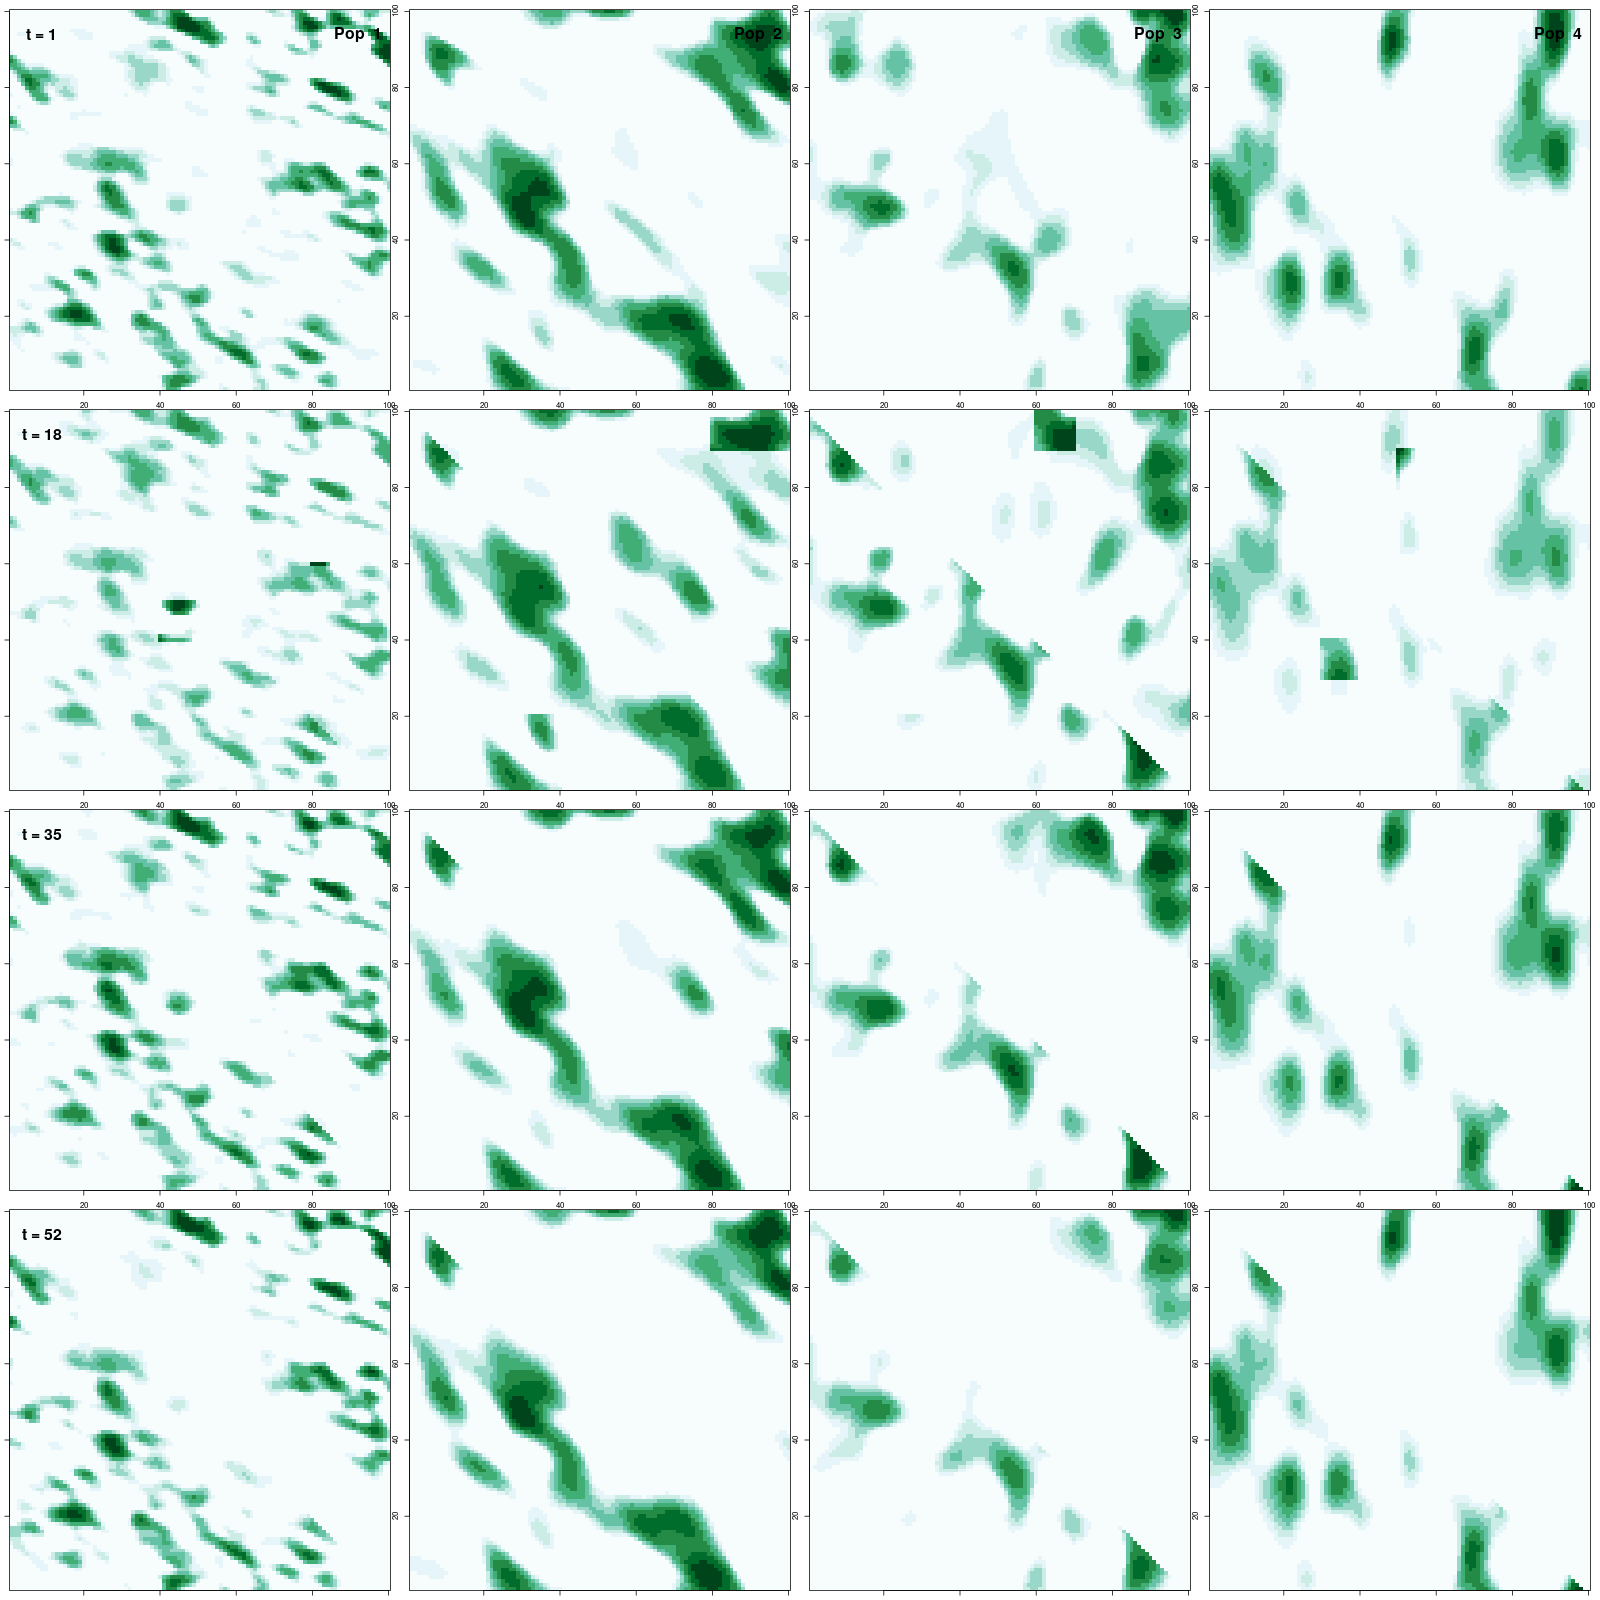
\includegraphics[width = \linewidth]{Plots/pop_dist}
	\caption{Spatial density (log abundance) for each of the four
		populations at four time steps. The darker the colour the
		greater the density of the population. Note that a diagonal
		anisotropic pattern (mimicking a depth gradient) can be
		clearly seen in populations 2 and 3. The concentrated spawning
		areas are also visible in the second row of the panels
		(t=18).}
	\label{fig:9}
\end{figure}	

\begin{figure}[!ht]
	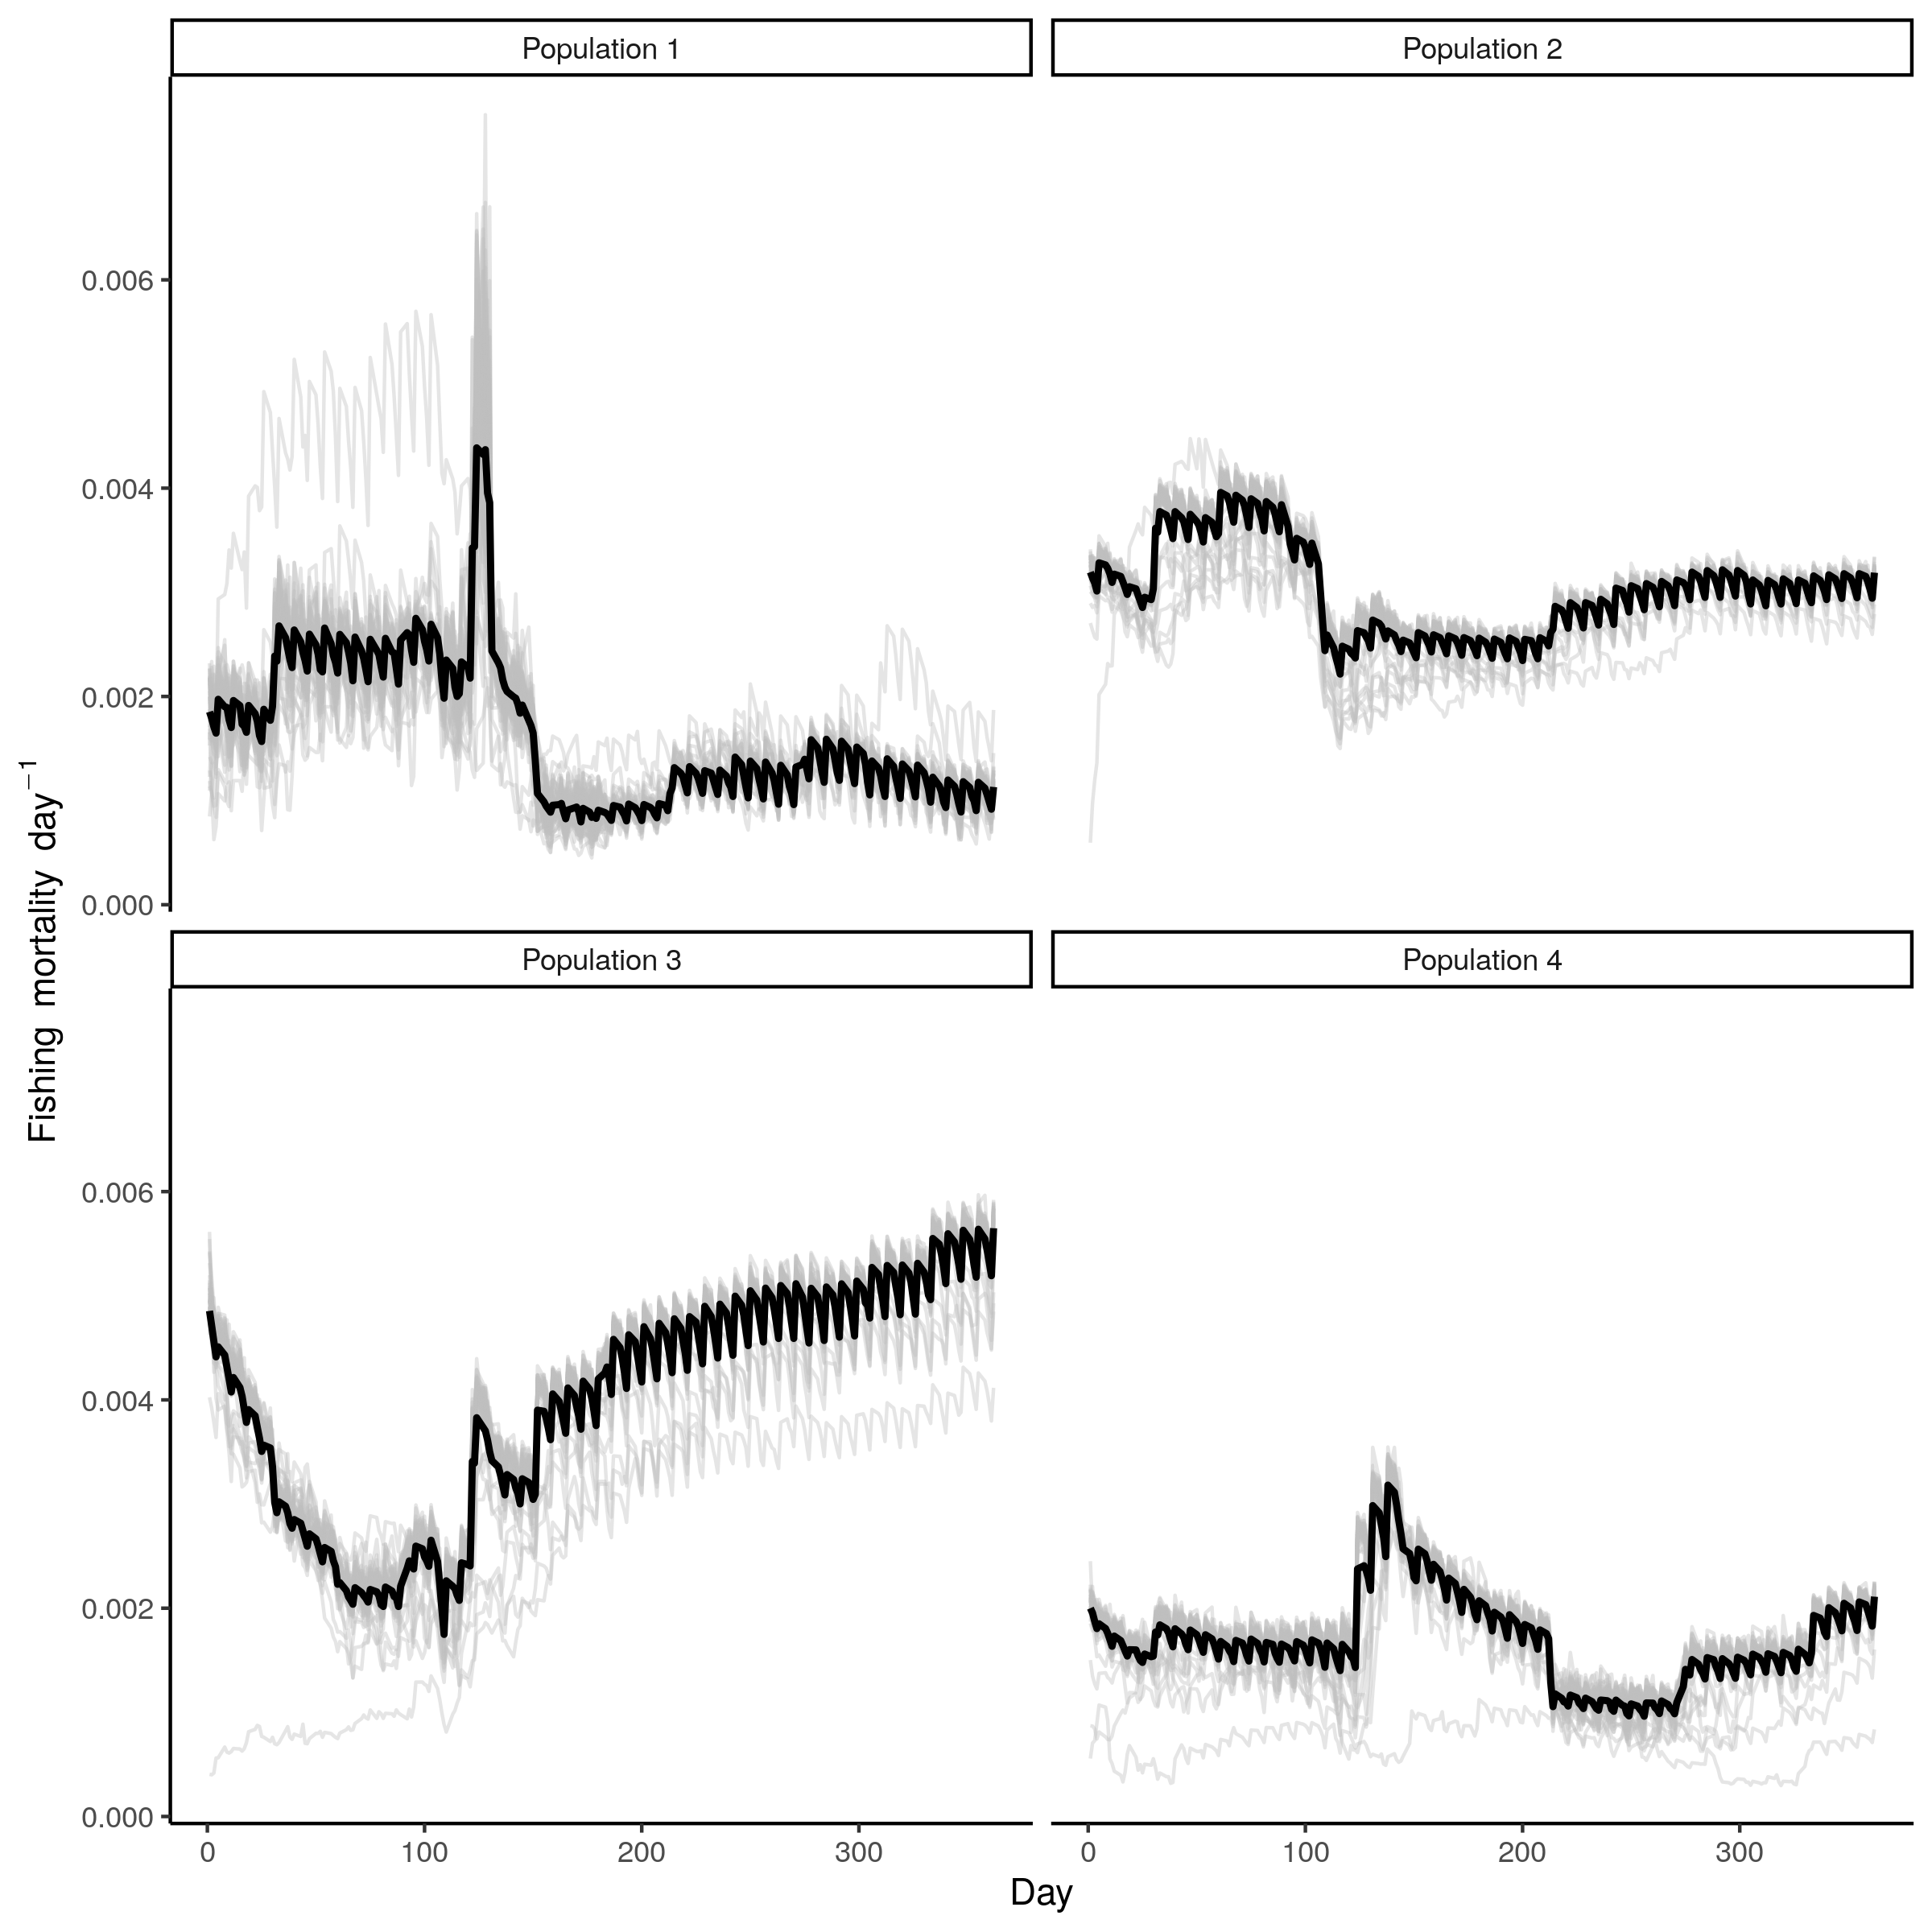
\includegraphics[width = \linewidth]{Plots/f_dynamics}
	\caption{Fishing mortality dynamics - the daily fishing mortalities
		aggregated across the entire spatial domain showing weekly and
		seasonal patterns in exploitation. Individual years are the
		light grey lines, the mean of all years the thick black line.}
	\label{fig:10}
\end{figure}	

\begin{figure}[!ht]
	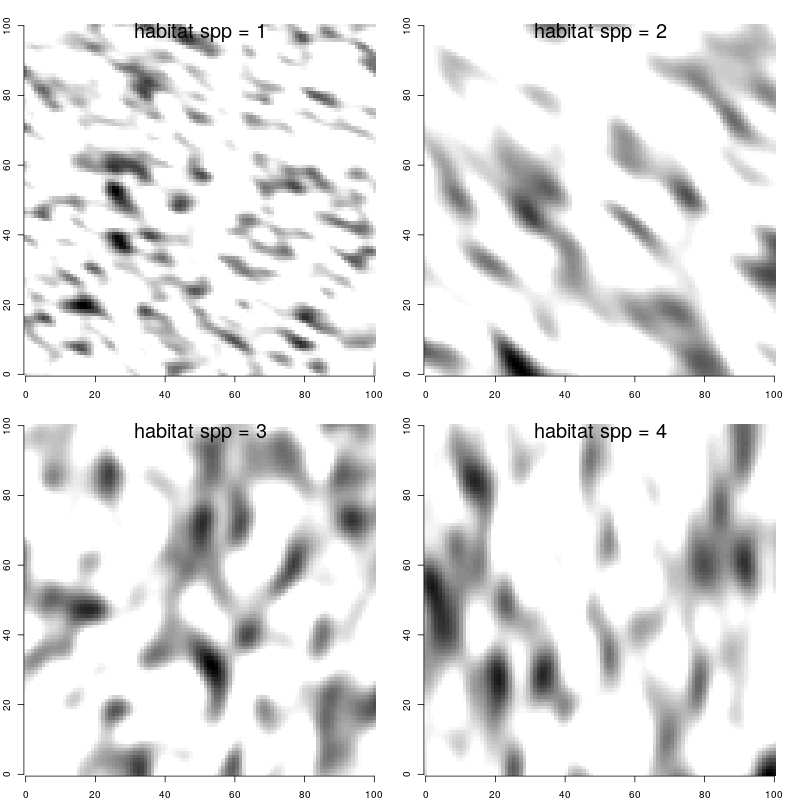
\includegraphics[width = \linewidth]{../analysis/habitat}
	\caption{Habitat preference: the distribution of suitable habitat for
		each population, with the darker colour showing greater
		habitat suitability.}
	\label{fig:1}
\end{figure}	

\begin{figure}[!ht]
	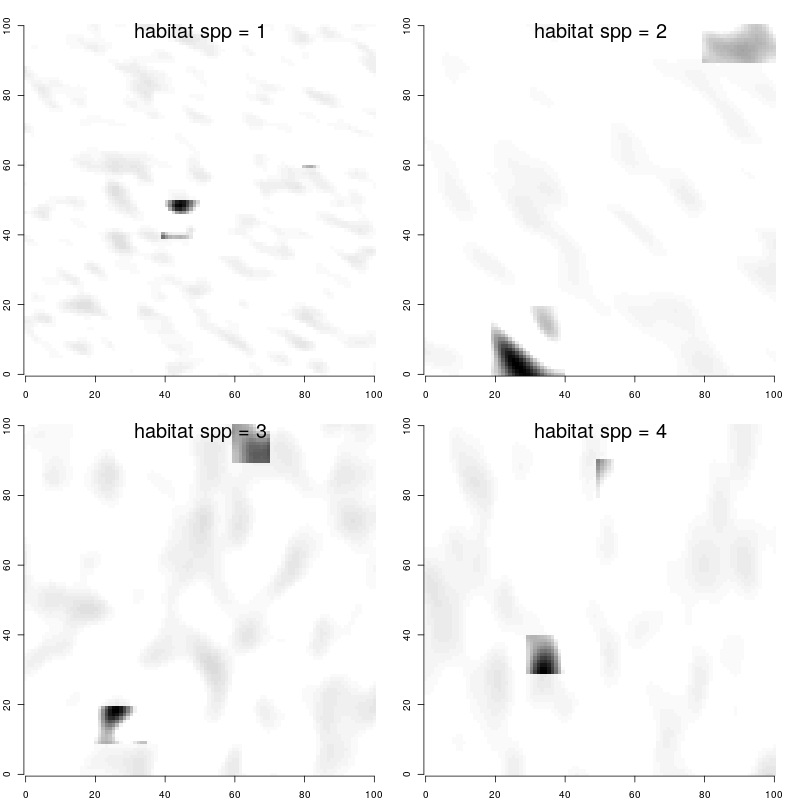
\includegraphics[width = \linewidth]{../analysis/habitat_spwn}
	\caption{Spawning habitat preference: the habitat suitability during
		spawning periods for each population. The darker the colour,
		the more suitable the habitat. The location of the spawning
		habitat is highlighted by the squares in each panel.}
	\label{fig:2}
\end{figure}	


\begin{figure}[!ht]
	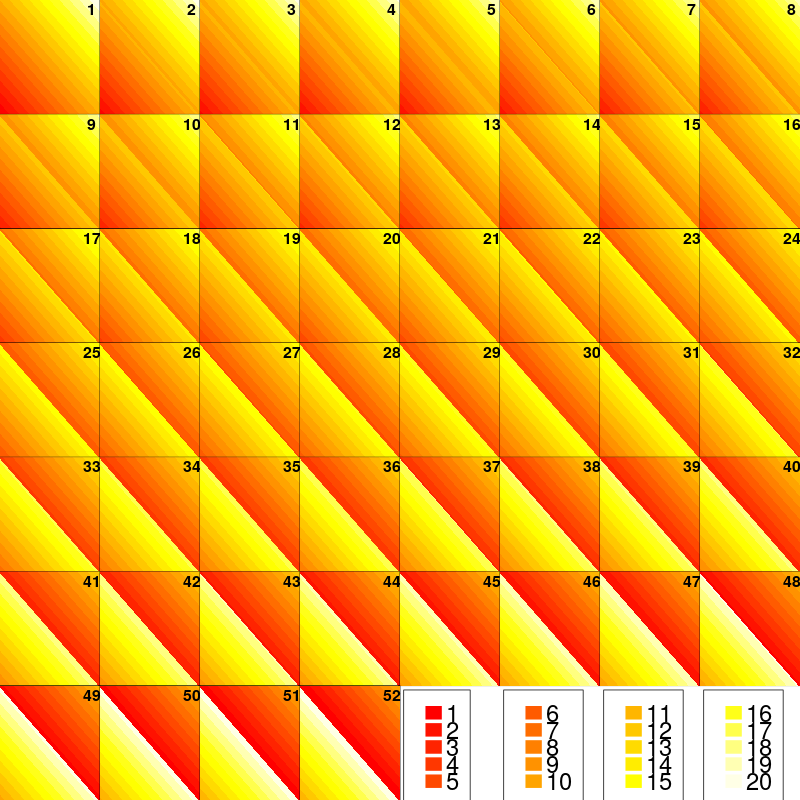
\includegraphics[width = \linewidth]{Plots/Temperature_gradient}
	\caption{Spatiotemporal temperature gradient: The temperature gradient
	for each time step (weeks, shown in top right corner of each panel.)}
	\label{fig:3}
\end{figure}

\begin{figure}[!ht]
	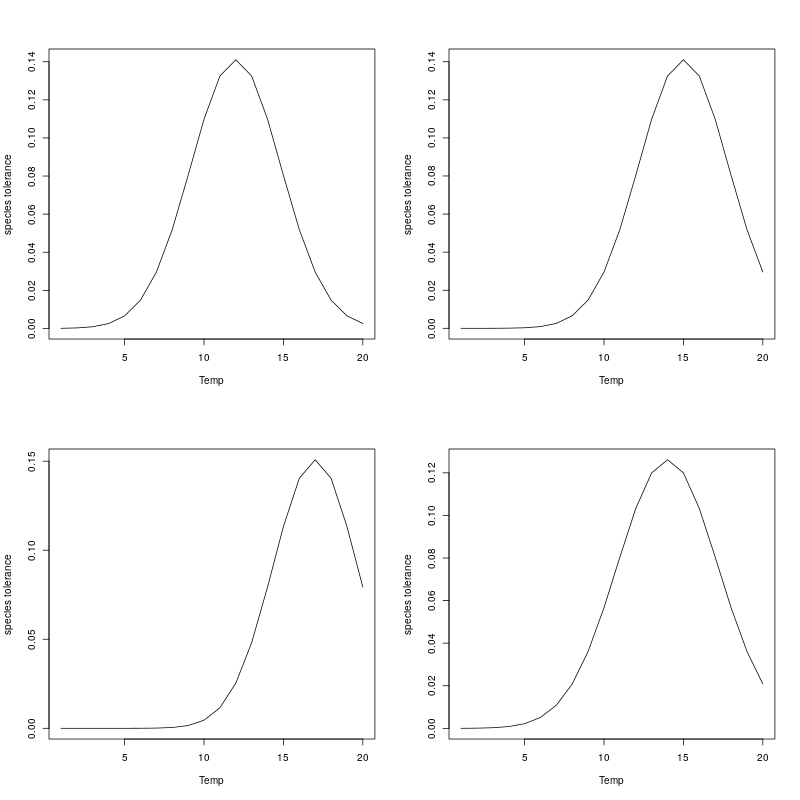
\includegraphics[width = \linewidth]{Plots/Species_tolerances}
	\caption{Species thermal tolerances: The tolerance of each population
		to different temperatures (x-axis) shown as a probability
		density function.}
	\label{fig:4}
\end{figure}

\begin{figure}[!ht]
	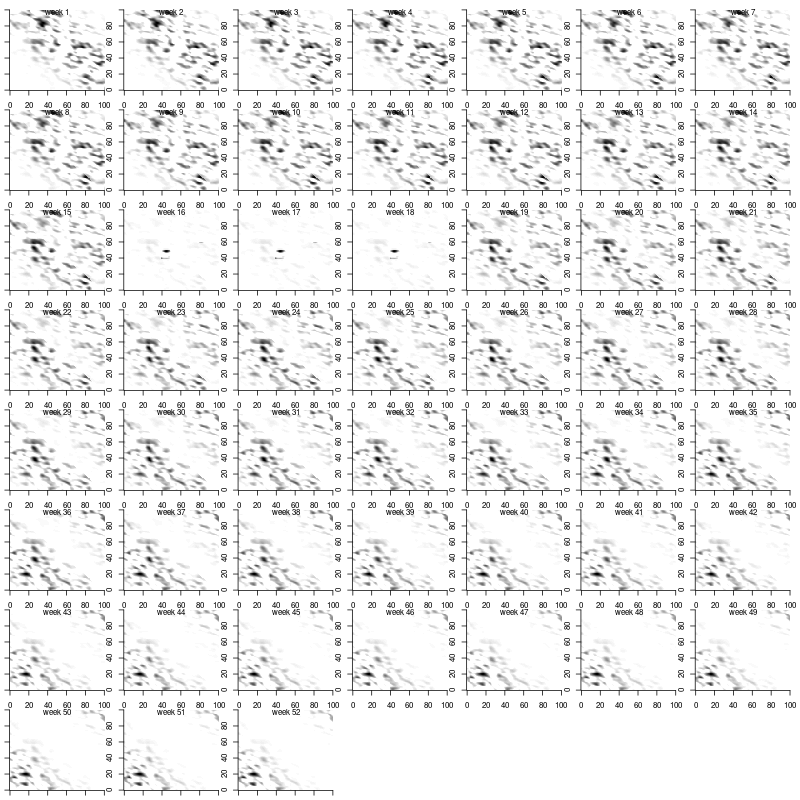
\includegraphics[width = \linewidth]{Plots/habitat_spatiotemp_spp_1}
	\caption{Spatiotemporal habitat suitability - the suitability habitat
		(for Population 1) for 52 separate weeks. The darker the
		colour, the more suitable the habitat for the population given
	the habitat and temperature tolerance.}
	\label{fig:5}
\end{figure}

\begin{figure}[!ht]
	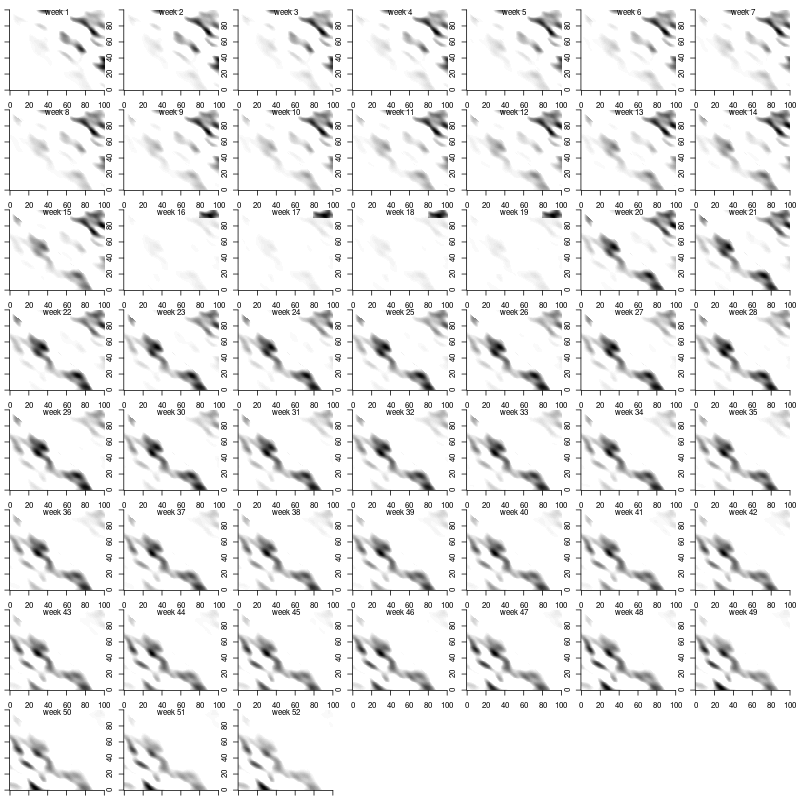
\includegraphics[width = \linewidth]{Plots/habitat_spatiotemp_spp_2}
	\caption{Spatiotemporal habitat suitability - the suitability habitat
		(for Population 2) for 52 separate weeks. The darker the
		colour, the more suitable the habitat for the population given
	the habitat and temperature tolerance.}
	\label{fig:6}
\end{figure}

\begin{figure}[!ht]
	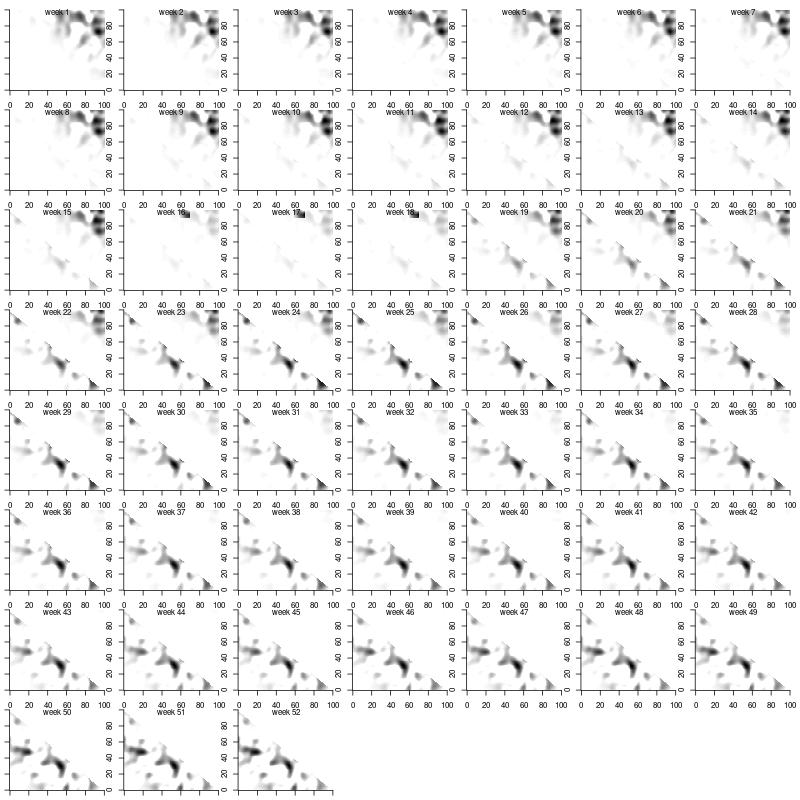
\includegraphics[width = \linewidth]{Plots/habitat_spatiotemp_spp_3}
	\caption{Spatiotemporal habitat suitability - the suitability habitat
		(for Population 3) for 52 separate weeks. The darker the
		colour, the more suitable the habitat for the population given
	the habitat and temperature tolerance.}
	\label{fig:7}
\end{figure}

\begin{figure}[!ht]
	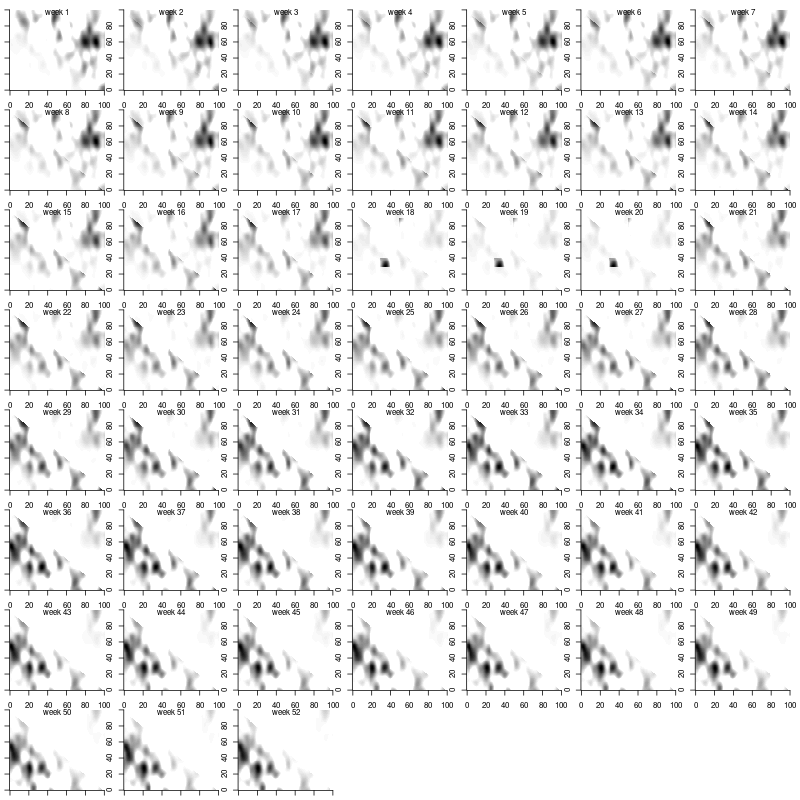
\includegraphics[width = \linewidth]{Plots/habitat_spatiotemp_spp_4}
	\caption{Spatiotemporal habitat suitability - the suitability habitat
		(for Population 4) for 52 separate weeks. The darker the
		colour, the more suitable the habitat for the population given
	the habitat and temperature tolerance.}
	\label{fig:8}
\end{figure}


\end{document}

